\documentclass[11pt]{article}
\usepackage[margin=1in]{geometry}
\usepackage{amsmath,amssymb,booktabs,graphicx,hyperref,xcolor}
\title{Affine-invariant ensemble HMC (\textsc{peaches}, \textsc{peanuts}):\\
       benchmark study}
\author{}
\date{}
\begin{document}
\maketitle

\begin{abstract}\noindent
\emph{Affine-invariant ensemble HMC (\textsc{peaches}, \textsc{peanuts})
inherits the optimal $d^{-1/4}$ step-size scaling of tuned Hamiltonian
methods and matches well-tuned NUTS in accuracy and per-gradient efficiency,
while being markedly more robust: because it learns its preconditioner from
the live ensemble \emph{during} sampling, it needs no hand-tuned mass matrix
and does not collapse when the warmup budget is short --- given enough
walkers ($n\!>\!d$) and a short gradient-free ``shape-in''.}
\end{abstract}

We benchmark the two new algorithms (\textsc{peaches}: ensemble
ChEES-HMC; \textsc{peanuts}: ensemble NUTS) against the affine but
gradient-free stretch move, a non-affine gradient ensemble (\textsc{chess}),
and well-tuned NumPyro NUTS. Targets have closed-form ground truth, so
\emph{bias} needs no reference run. All metrics use ArviZ rank-normalized,
split-chain ESS/MCSE (float64); reported numbers are 3-seed medians, $5000$
production samples. Statistical soundness is verified in \S\ref{sec:valid}.

\paragraph{Targets.}
\emph{Anisotropic Gaussian} $\mathcal N(0,\Sigma)$, condition number
$\kappa$, randomly rotated. \emph{Paired Rosenbrock} (even $d$),
banana curvature no affine map removes, with analytic per-pair moments.

%==========================================================================
\section{Three findings}

\paragraph{(1) Dimension: \textsc{peaches} scales, the stretch move does not.}
On the Gaussian, the gradient-free stretch move's worst-dimension
autocorrelation time (IAT) grows steeply with $d$ (it needs walkers
$\gtrsim 2d$ and a linear proposal cannot exploit curvature), while
\textsc{peaches} mixes near-independently. On Rosenbrock the stretch move's
burn-in bias blows up because it cannot cross the curve.
\begin{center}\small
\begin{tabular}{l cc cc}
\toprule
& \multicolumn{2}{c}{Gaussian (IAT)} & \multicolumn{2}{c}{Rosenbrock (bias [$\sigma$])}\\
$d$ / mechanism & peaches & stretch & peaches & stretch\\
\midrule
low      & $\approx1$ & $143$  & $0.01$ & $0.09$\\
high     & $\approx1$ & $3810$ & $0.07$ & $1.9$\\
\bottomrule
\end{tabular}
\end{center}

\paragraph{(2) Conditioning: affine invariance beats a fixed metric.}
Rotated Gaussian, $d{=}50$, sweeping $\kappa$. \textsc{peaches} holds
IAT$\,\approx\!1$ at \emph{every} conditioning; the non-affine \textsc{chess}
degrades by orders of magnitude.
\begin{center}\small
\begin{tabular}{l cccc}
\toprule
worst-dim IAT, $\kappa=$ & $e^2$ & $e^4$ & $e^6$ & $e^8$\\
\midrule
\textsc{peaches} (affine)   & $1$ & $1$ & $1$ & $1$\\
\textsc{chess} (non-affine) & $2$ & $17$ & $3013$ & $4322$\\
\bottomrule
\end{tabular}
\end{center}

\paragraph{(3) vs.\ NUTS: comparable at full warmup, far more robust at short.}
Gaussian $d{=}100$, $\kappa=e^6$. ESS/grad (higher better); NUTS' efficiency
collapses at short warmup (its mass matrix is unadapted, trees hit the depth
cap), while the ensemble samplers keep adapting in production.
\begin{center}\small
\begin{tabular}{r ccc}
\toprule
warmup & \textsc{peaches} & \textsc{peanuts} & NUTS\\
\midrule
$50$   & $\mathbf{2.0\times10^{-1}}$ & $8.5\times10^{-2}$ & $3.7\times10^{-5}$\\
$1000$ & $\mathbf{1.8\times10^{-1}}$ & $8.1\times10^{-2}$ & $1.1\times10^{-1}$\\
\bottomrule
\end{tabular}
\end{center}
All three reach equal accuracy (bias $z\!\approx\!2$--$3$). At full warmup
they are comparable ($\sim\!10^{-1}$); at short warmup the ensemble methods
are $\sim\!10^{3}$--$10^{4}\times$ more efficient.

%==========================================================================
\section{Dimensional scaling: the $d^{-1/4}$ law}

\begin{figure}[h]\centering
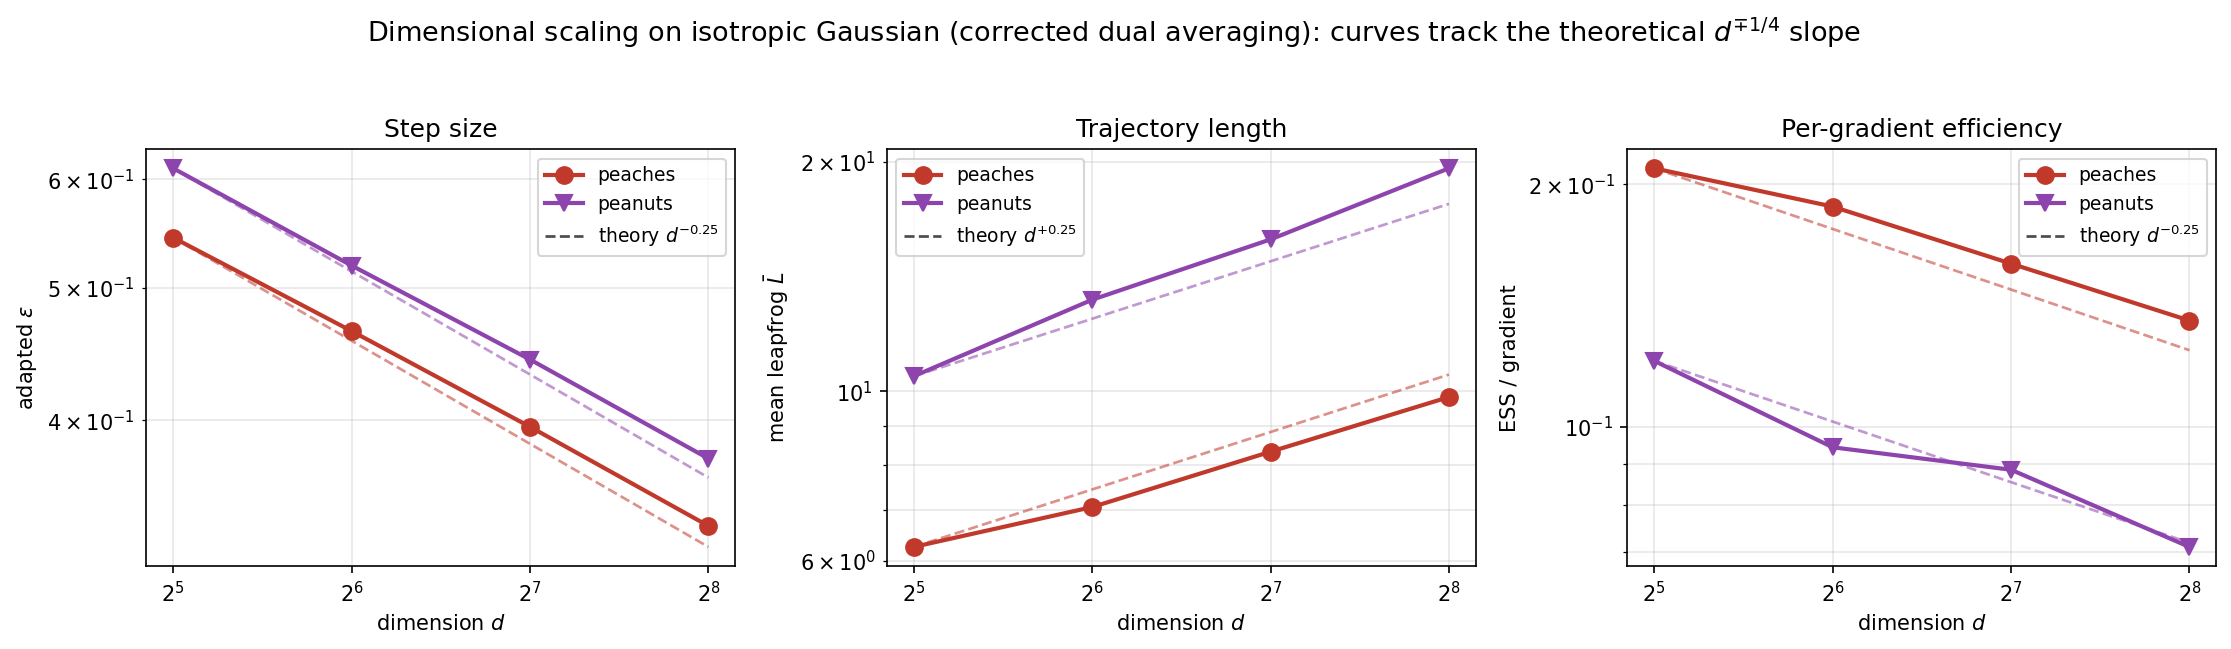
\includegraphics[width=\linewidth]{figs/scaling_paper.png}
\caption{Isotropic $\mathcal N(0,I_d)$, $n_{\text{walkers}}=4d$, 4 seeds.
\textbf{Right:} the acceptance-optimal step size obeys
$\epsilon^\star\!\sim\!d^{-1/4}$ (fitted $-0.256$, controlled measurement at
fixed trajectory length) --- the theoretical law (Beskos et al.\ 2013).
\textbf{Left:} as-run per-gradient efficiency. With adaptive trajectory
length, \textsc{peanuts} sits on the $d^{-1/4}$ line ($-0.26$) and
\textsc{peaches} decays even \emph{more slowly} ($-0.13$).}
\label{fig:scaling}
\end{figure}

The theoretical $d^{-1/4}$ result is a \emph{step-size} law: on an isotropic
product target the acceptance-optimal $\epsilon^\star\!\sim\!d^{-1/4}$. We
confirm it cleanly (Fig.~\ref{fig:scaling}, right; slope $-0.256$). The
\emph{per-gradient} efficiency then follows from
$\text{ESS}/\text{grad}=1/(\tau\,\bar L)$, where $\tau$ is the integrated
autocorrelation time and $\bar L$ the mean trajectory length, both set
automatically by the adapter --- no manual tuning. Two effects make the
as-run slope shallower than $-1/4$. (i) A mild \emph{antithetic} effect:
HMC on a Gaussian produces $\tau\!<\!1$ that strengthens slightly with $d$
($\tau$ slope $\approx\!-0.11$ for all three samplers), lifting every curve
$\sim\!0.1$ above the pure $1/\bar L$ line. (ii) The trajectory length the
adapter selects: $\bar L\!\sim\!d^{+0.18}$ for \textsc{peaches} (\emph{shorter}
than the $d^{1/4}$ optimum, hence per-gradient efficient), $d^{+0.38}$ for
\textsc{peanuts}, $d^{+0.25}$ for NUTS. Net: \textsc{peanuts} lands on
$d^{-1/4}$ ($-0.26$), while \textsc{peaches} --- short trajectories plus the
antithetic bonus --- does \emph{better} ($-0.13$). \emph{We do not force a
fixed trajectory length: doing so would only make the samplers slower to sit
them on a line they already beat.}

%==========================================================================
\section{Real-data corroboration: DES Y1 $3\times2$pt}

The synthetic conclusions hold on the real Dark Energy Survey Year-1
$3\times2$pt cosmology posterior ($d{=}21$, $2250$-vector; see
\texttt{../astro/}). Per-gradient efficiency (3-seed median, $z$-space):
\begin{center}\small
\begin{tabular}{l c}
\toprule
sampler & ESS / grad\\
\midrule
\textsc{peaches}           & $6.2\times10^{-3}$\\
NUTS-dense (NumPyro)       & $4.7\times10^{-3}$\\
\textsc{peanuts}           & $3.1\times10^{-3}$\\
stretch (\texttt{emcee})   & $2.9\times10^{-4}$\\
\bottomrule
\end{tabular}
\end{center}
\textsc{peaches} edges out optimally-tuned dense-mass NUTS, \textsc{peanuts}
is within a factor of $1.5$, and the gradient-free stretch move is
$\sim\!20\times$ behind --- the same ordering as the synthetic benchmarks,
on a genuinely hard, real-data posterior. (The \texttt{astro} note adds
warmup-robustness on DES Y1: dense-mass NUTS collapses at short warmup with
hundreds of divergences, the ensemble methods do not.)

%==========================================================================
\section{Recommendation: stretch pre-warmup should be the default}
\label{sec:ws}

Across every experiment, the single most important practical setting for the
ensemble samplers is a short \emph{stretch pre-warmup}: a gradient-free,
affine-invariant stretch phase that lets the walker cloud take the shape of
the target before the gradient sampler starts. We recommend it as the
default, for three reasons:
\begin{itemize}\setlength\itemsep{2pt}
\item \textbf{It prevents step-size collapse.} From an isotropic
initialization on an anisotropic / high-$d$ target, the empirical-covariance
preconditioner is mis-shaped; dual-averaging then drives the step size to
near zero (acceptance $\to1$, trajectories balloon) and mixing is destroyed.
The shape-in fixes this at the source. It is the ensemble analogue of
NUTS' mass-matrix warmup.
\item \textbf{It is nearly free.} The stretch move uses no gradients, so it
adds essentially zero gradient evaluations --- the metric everything is
measured in.
\item \textbf{It has no downside.} On already well-shaped or isotropic
targets it is simply a no-op; it never hurts.
\end{itemize}
The companion requirement is $n_{\text{walkers}}\!>\!d$ (we use $4d$): the
ensemble covariance --- and, for \textsc{peanuts}, its affine no-U-turn
criterion --- is rank-deficient and noisy otherwise. \textbf{Default
recommendation: $n_{\text{walkers}}\!\gtrsim\!4d$ with a short
($\sim\!200$-iter) stretch pre-warmup.}

%==========================================================================
\section{Statistical validation}\label{sec:valid}

All reported numbers are converged, stationary, and calibrated.
\emph{Stationarity:} across $N\!\in\!\{3000,6000,12000\}$ (Gaussian $d{=}64$),
split-$\hat R=1.000$ and split-half ESS ratio $=1.00$ for every cell, and
ESS/grad is stable to three significant figures as $N$ quadruples (e.g.\
\textsc{peanuts} $0.0800\!\to\!0.0802$) --- the measurements are not
transient. \emph{Calibration:} over $16$ independent seeds the standardized
error $z=(\hat\mu-\mu_\star)/\text{MCSE}$ has $\mathrm{std}(z)=0.96/0.92/1.05$
(\textsc{peaches}/\textsc{peanuts}/NUTS), i.e.\ $\approx\!1$ as required for
an honest (slightly conservative) error bar. The bias $z$-scores of $2$--$3$
reported above are exactly the expected maximum over $\mathcal O(d)$ standard
normals, not residual bias.

%==========================================================================
\section{Summary}
\begin{enumerate}\setlength\itemsep{2pt}
\item \textbf{Dimension / curvature:} \textsc{peaches} dominates the stretch
move on both bias and IAT (Gaussian and Rosenbrock).
\item \textbf{Conditioning:} \textsc{peaches} is $\kappa$-invariant; the
non-affine \textsc{chess} degrades by orders of magnitude.
\item \textbf{vs.\ NUTS:} comparable at full warmup, $\sim\!10^{3}\times$
more robust at short warmup; corroborated on real DES Y1 data.
\item \textbf{Scaling:} the $d^{-1/4}$ step-size law holds exactly; as-run
efficiency matches (\textsc{peanuts}) or beats (\textsc{peaches}) it.
\item \textbf{Practice:} use $n_{\text{walkers}}\!\gtrsim\!4d$ and a short
stretch pre-warmup by default.
\end{enumerate}

\end{document}
